
%(BEGIN_QUESTION)
% Copyright 2011, Tony R. Kuphaldt, released under the Creative Commons Attribution License (v 1.0)
% This means you may do almost anything with this work of mine, so long as you give me proper credit

Suppose two radio transceivers must communicate with each other over a long distance.  Each one uses a half-wave ``whip'' antenna with 6 dBi gain, a lightning arrestor at the transceiver ($-0.5$ dB loss at each transceiver), and each one has 25 feet of coaxial cable connecting the transceiver to the antenna ($-0.2$ dB loss per foot).  Each transceiver transmits 350 mW of RF power, and has a receiving sensitivity of $-103$ dBm. 

Assuming a 900 MHz signal frequency, no fade loss, and absolutely clear line-of-sight between the two antennas, how far away may these transceivers be separated and still fall within the RF budget for good communication?

\vfil 

\underbar{file i03396}
\eject
%(END_QUESTION)





%(BEGIN_ANSWER)

This is a graded question -- no answers or hints given!

%(END_ANSWER)





%(BEGIN_NOTES)

A good problem-solving technique to apply here is to sketch a picture of the system, labeling it with all the given data:

$$\includegraphics[width=15.5cm]{i03396x01.eps}$$

It looks like the only unknown in this problem is the path loss: how much power we will be allowed to lose over the distance between antennas due to signal spreading while still allowing the receiver to gets its requisite power level.

To begin our calculation, we should convert the transmitter's 350 mW power value into dBm so that it matches units with all the other figures given to us:

$$10 \log \left(350 \hbox{ mW} \over 1 \hbox{ mW}\right) = 25.44 \hbox{ dBm}$$

From this source power, we are allowed to lose 128.44 dB of signal (from 25.44 dBm at the transmitter all the way down to $-103$ dBm at the receiver input).  Totaling the given losses in cables, arrestors, and making up slightly in antenna gains:

$$(25 \hbox{ ft})(-0.2 \hbox{ dB/ft}) + (-0.5 \hbox{ dB}) + 6 \hbox{ dB} + 6 \hbox{ dB} + (-0.5 \hbox{ dB}) + (25 \hbox{ ft})(-0.2 \hbox{ dB/ft}) = +1 \hbox{ dB}$$

Thus, our allowable path loss is $-129.44$ dB (the allowed total power loss of $-128.44$ dB plus the slight gain of the whip antennas plus cables and arrestors).  Knowing the path loss figure in decibels allows us to calculate distance, but first we must calculate the wavelength of this radio signal based on ferquency:

$$\lambda = {2.9979 \times 10^8 \over 900 \times 10^6} = 0.3331 \hbox{ m}$$

\filbreak

Manipulating the path loss equation to solve for distance ($D$):

$$L_p = -20 \log \left( 4 \pi D \over \lambda \right)$$

$${L_p \over -20} = \log \left( 4 \pi D \over \lambda \right)$$

$$10^{\left({L_p \over -20}\right)} = {4 \pi D \over \lambda}$$

$$\lambda 10^{\left({L_p \over -20}\right)} = 4 \pi D$$

$${{\lambda 10^{\left({L_p \over -20}\right)}} \over 4 \pi} = D$$

Now, plugging in our known values for path loss and lambda:

$${{0.3331 \times 10^{\left({-129.44 \over -20}\right)}} \over 4 \pi} = 78.596 \hbox{ km}$$

\vskip 10pt

Thus, the maximum distance is 78.596 kilometers, or 48.84 miles.

%INDEX% Electronics review, RF link budget calculation

%(END_NOTES)


